\documentclass[journal]{IEEEtran}
\usepackage[a5paper, margin=10mm, onecolumn]{geometry}
\usepackage{lmodern}
\usepackage{tfrupee}
\setlength{\headheight}{1cm}
\setlength{\headsep}{0mm}

\usepackage{gvv-book}
\usepackage{gvv}
\usepackage{cite}
\usepackage{amsmath,amssymb,amsfonts,amsthm}
\usepackage{algorithmic}
\usepackage{graphicx}
\usepackage{textcomp}
\usepackage{xcolor}
\usepackage{txfonts}
\usepackage{listings}
\usepackage{enumitem}
\usepackage{mathtools}
\usepackage{gensymb}
\usepackage{comment}
\usepackage[breaklinks=true]{hyperref}
\usepackage{tkz-euclide}
\usepackage{listings}
\def\inputGnumericTable{}
\usepackage[latin1]{inputenc}
\usepackage{color}
\usepackage{array}
\usepackage{longtable}
\usepackage{calc}
\usepackage{multirow}
\usepackage{hhline}
\usepackage{ifthen}
\usepackage{lscape}
\usepackage{xparse}

\bibliographystyle{IEEEtran}

\title{4.13.47}
\author{EE25BTECH11043 - Nishid Khandagre} % Replace with your name

\begin{document}
\maketitle

\renewcommand{\thefigure}{\theenumi}
\renewcommand{\thetable}{\theenumi}

\numberwithin{equation}{enumi}
\numberwithin{figure}{enumi}

\textbf{Question}:
The ends $\vec{A}$, $\vec{B}$ of a straight line segment of constant length $c$ slide upon the fixed rectangular axes $OX$, $OY$ respectively. If the rectangle $OAPB$ be completed, then show that the locus of the foot of perpendicular drawn from $\vec{P}$ to $\vec{AB}$ is
\[x^{\frac{2}{3}} + y^{\frac{2}{3}} = c^{\frac{2}{3}}\]

\textbf{Solution:}


Given
\begin{align}
\vec{A} &= \myvec{a\\0} \\
\vec{B} &= \myvec{0\\b}
\end{align}
Since $OAPB$ is a rectangle, the opposite corner $\vec{P}$ is:
\begin{align}
\vec{P} &= \vec{A} + \vec{B} \\
&= \myvec{a \\ b}
\end{align}
$\vec{B}-\vec{A}$ has fixed length of $c$
\begin{align}
\norm{\vec{B}-\vec{A}}^2 &= \myvec{\vec{B}-\vec{A}}^\top\myvec{\vec{B}-\vec{A}} \\
c^2&= a^2+b^2
\end{align}
Let $\vec{H}$ be the foot of the perpendicular from $\vec{P}$ to the line through $\vec{A}$ in the direction $\vec{B}-\vec{A}$.
\begin{align}
\vec{H} &= \vec{A} + \lambda\myvec{\vec{B}-\vec{A}} \\
\lambda &= \frac{\myvec{\vec{P}-\vec{A}}^\top\myvec{\vec{B}-\vec{A}}}{\myvec{\vec{B}-\vec{A}}^\top\myvec{\vec{B}-\vec{A}}}
\end{align}

\begin{align}
\vec{P}-\vec{A} &= \myvec{\vec{A}+\vec{B}}-\vec{A} \\
&= \vec{B}
\end{align}
So,
\begin{align}
\lambda &= \frac{\vec{B}^\top\myvec{\vec{B}-\vec{A}}}{\myvec{\vec{B}-\vec{A}}^\top\myvec{\vec{B}-\vec{A}}} \\
&= \frac{\vec{B}^\top\vec{B}-\vec{B}^\top\vec{A}}{a^2+b^2}
\end{align}
We know
\begin{align}
\vec{B}^\top\vec{A}=0\\
\vec{B}^\top\vec{B}=b^2
\end{align}
\begin{align}
\lambda &= \frac{b^2}{a^2+b^2}
\end{align}
Now compute $\vec{H}$:
\begin{align}
\vec{H} &= \vec{A} + \frac{b^2}{a^2+b^2}\myvec{\vec{B}-\vec{A}}\\
&= \myvec{a\\0} + \frac{b^2}{a^2+b^2}\myvec{-a\\b} \\
&= \myvec{a - \frac{ab^2}{a^2+b^2} \\ \frac{b^3}{a^2+b^2}} \\
&= \myvec{\frac{a(a^2+b^2)-ab^2}{a^2+b^2} \\ \frac{b^3}{a^2+b^2}} \\
&= \myvec{\frac{a^3}{a^2+b^2} \\ \frac{b^3}{a^2+b^2}}
\end{align}
Let $\vec{H} = \myvec{x \\ y}$. Then,
\begin{align}
x &= \frac{a^3}{a^2+b^2} \\
y &= \frac{b^3}{a^2+b^2}
\end{align}
Using the constraint $a^2+b^2=c^2$:
\begin{align}
a^3 &= x(a^2+b^2) = xc^2 \\
b^3 &= y(a^2+b^2) = yc^2
\end{align}
Thus,
\begin{align}
a &= (xc^2)^{1/3} = c^{2/3}x^{1/3} \\
b &= (yc^2)^{1/3} = c^{2/3}y^{1/3}
\end{align}
Substitute these into $a^2+b^2=c^2$:
\begin{align}
(c^{2/3}x^{1/3})^2 + (c^{2/3}y^{1/3})^2 &= c^2 \\
c^{4/3}x^{2/3} + c^{4/3}y^{2/3} &= c^2 \\
c^{4/3}(x^{2/3} + y^{2/3}) &= c^2
\end{align}
The locus is:
\begin{align}
x^{2/3} + y^{2/3} &= c^{2/3}
\end{align}
\begin{figure}[H]
\centering
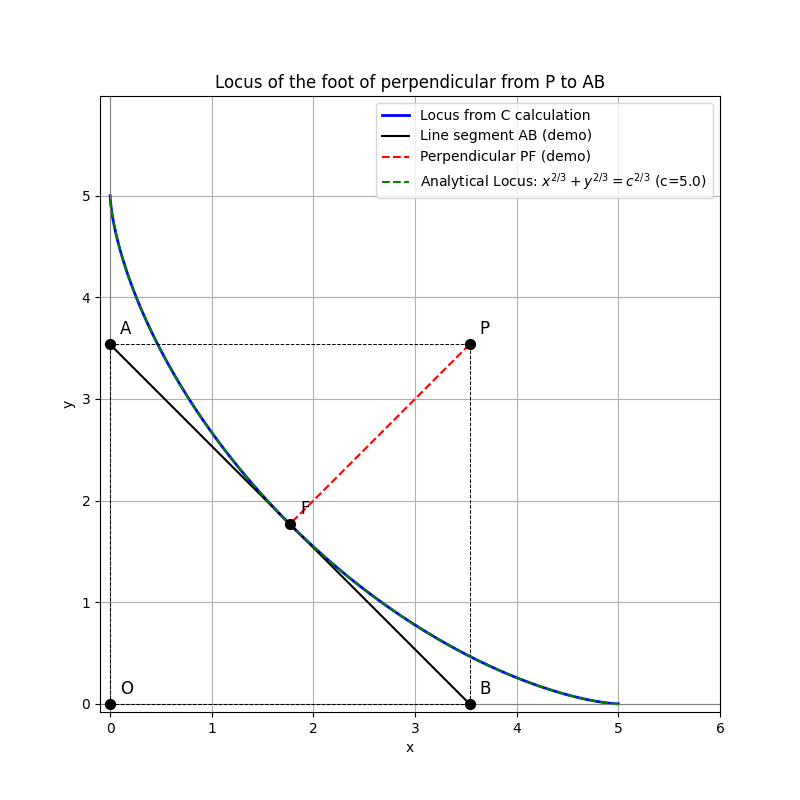
\includegraphics[width=0.7\columnwidth]{figs/fig1.png}
\caption{}
\label{fig:1}
\end{figure}

\end{document}
